\label{feeddown}
\begin{comment}
\begin{figure}
\centering
%\includegraphics[width=.49\linewidth]{figures/xxxxxxx}
%\includegraphics[width=.49\linewidth]{figures/xxxxxxx}
%\includegraphics[width=.49\linewidth]{figures/xxxxxxx}
 \caption{Top left: azimuthal correlation distribution between D meson from b-hadron decay and charged particles obtained from a Monte Carlo simulation
based on Pythia (Perugia-0 tune) fitted with a 2+1 Gaussian + constant function. The violet histogram is the template obtained by scaling the baseline
in order to match that measured in data. Top right: data correlation distributions obtained after the subtraction of the feed-down component, using 3 different values of $f_{\rm prompt}$ resulting
from the variation of the charm and beauty quark masses and factorization and renormalization scales employed in the FONLL calculation. Bottom: ratios between the azimuthal
distribution obtained with the maximum and minimum $f_{\rm prompt}$ values and that obtained with the central $f_{\rm prompt}$ value.}
 \label{fig:feeddownDescription}
\end{figure}
\end{comment}
%
%
The contribution of correlations of D meson from b-hadron decay is subtracted from the data correlation distributions as:
\begin{equation}
\tilde{C}_{\rm prompt~D}(\Delta\varphi)=\frac{1}{f_{\rm prompt}}\left(\tilde{C}_{\rm inclusive}(\Delta\varphi)-(1-f_{\rm prompt})\tilde{C}_{\rm feed-down}^{\rm MC~templ}(\Delta\varphi) \right).
\label{eqFeedDown}
\end{equation}
In the above equation, $\tilde{C}_{\rm inclusive}(\Delta\varphi)$ and $\tilde{C}_{\rm prompt~D}(\Delta\varphi)$ are per-trigger azimuthal correlation distributions before and after
feed-down contribution subtraction, $f_{\rm prompt}$ is the fraction of prompt D meson and $\tilde{C}_{\rm feed-down}^{\rm MC~templ}$ is a template
of the azimuthal correlation distribution for the feed-down component obtained from home-made Monte Carlo simulation at generated level, using PYTHIA6 with Perugia2011 tune.
In order to avoid biases related to the different event multiplicity in real and simulated events, the correlation distribution was shifted to have its minimum coinciding with the baseline of the data azimuthal-correlation distribution before feed-down subtraction. %[THIS HELD FOR pp...]A difference smaller than 8\% was observed in the simulation between the baseline values of the azimuthal-correlation distributions for prompt and feed-down D mesons. Considering the typical values of $f_{\rm prompt}$, this difference results in a shift of the baseline of $\tilde{C}_{\rm prompt~D}(\Delta\varphi$ of less than 1\%, negligible with respect to the other uncertainties affecting the measurement.

The value of $f_{\rm prompt}$ (Figure \ref{fprompt}), which depends on D-meson species and varies as a function of the $\pt$, is estimated on the basis of FONLL predictions for the production of feed-down D mesons at central rapidity, in pp collisions at $\sqrt(s) = 5$ TeV, and using the reconstruction efficiency of prompt and feed-down D mesons, following the so-called $N_{\rm b}$ approach defined in~\cite{ALICEDmespp7Tev}. Typical values ranges are about 8-10\% for the
$\Dzero$, about 4-7\% for the $\Dplus$ and about 5-8\% for the $\Dstar$. The procedure adopted is the same as what done in pp: however, in p--Pb, in order to consider a possible non-zero $v_{2}$-like modulation of the baseline, a range of $0<v_{2}<0.2$ values for tracks and for secondary D mesons is considered for the systematic uncerainty evaluation (using an hypothesis of no modulation for both cases for central values).

\begin{figure}
\centering
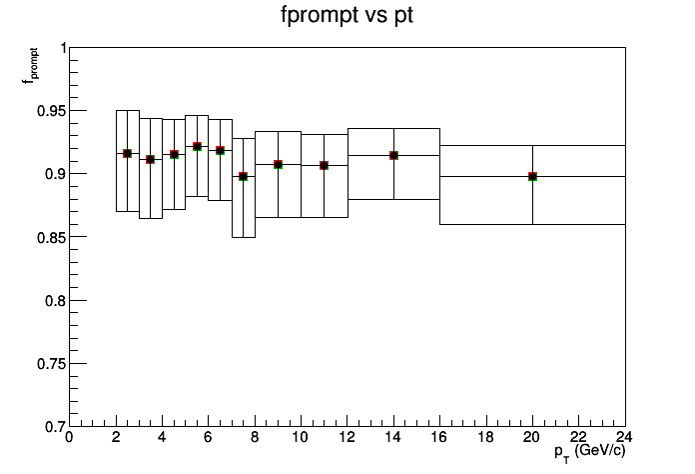
\includegraphics[width=0.6\linewidth]{figures/Effs/fprompt_D0.png}
\includegraphics[width=0.6\linewidth]{figures/Effs/fprompt_Dstar.png}
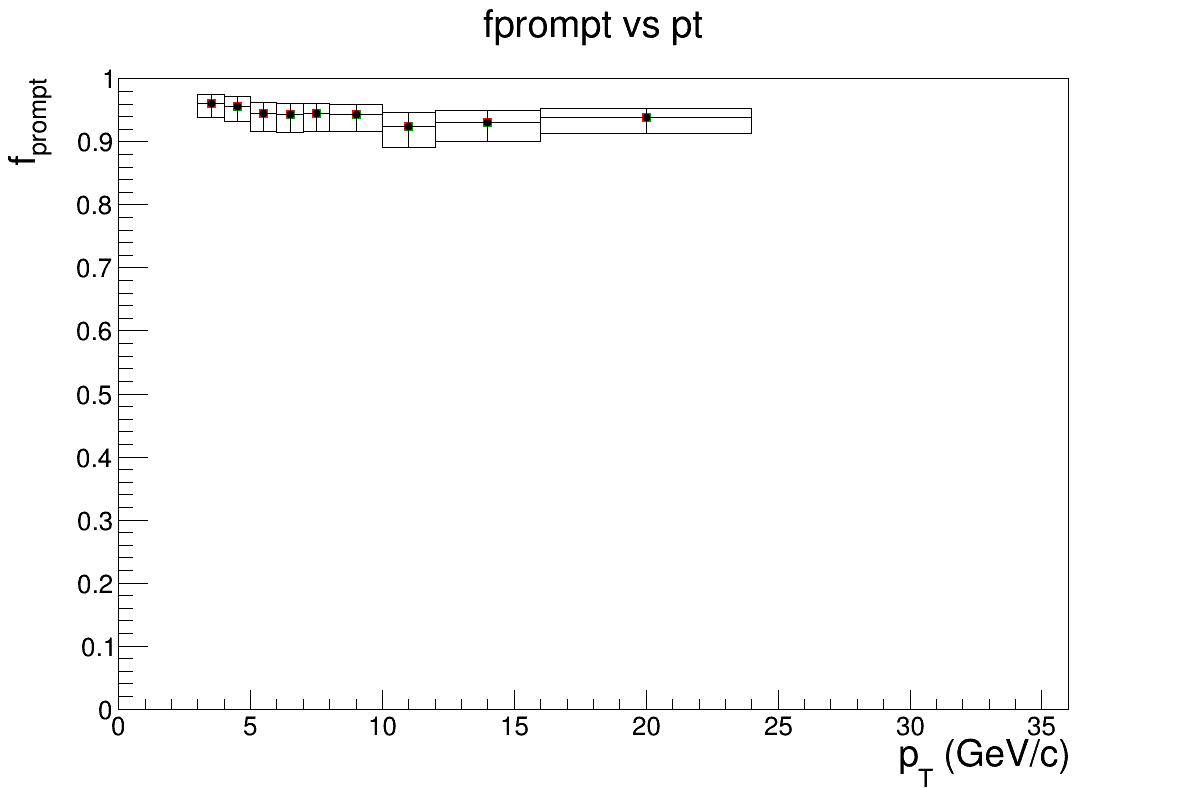
\includegraphics[width=0.6\linewidth]{figures/Effs/fpromptDplus.png}
\caption{$f_{\rm prompt}$ as a function of the $\pt$ for $\Dzero$ (top), $\Dstar$ (mid) and $\Dplus$ (bottom) estimated on the basis of FONLL predictions}
\label{fprompt}
\end{figure}

Examples of the PYTHIA templates used for the feed-down contribution subtraciton are shown in Figures \ref{templates1} (Figure \ref{templates2} shows the same templates but for prompt D mesons).

\begin{figure}
\centering
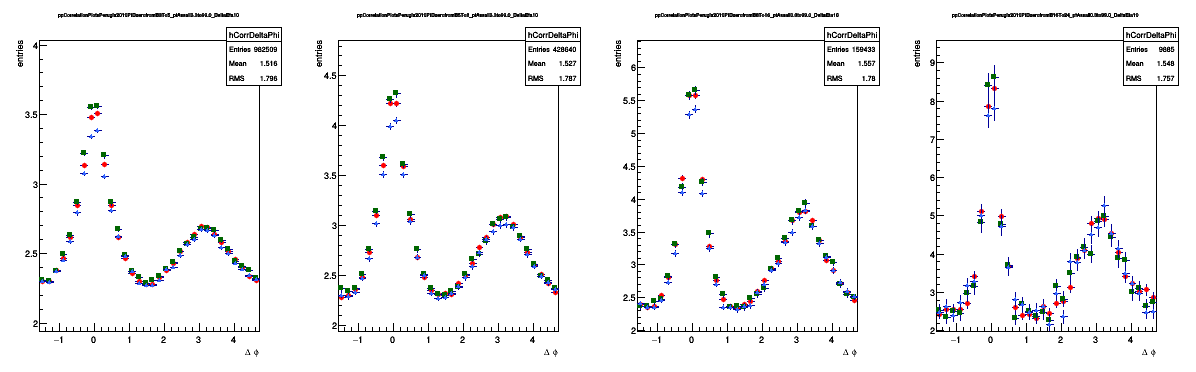
\includegraphics[width=1\linewidth]{figures/Template/1DCompare_allDpTfromB_AssoPt_0dot3to99dot0GeVc_Perugia2010.png}
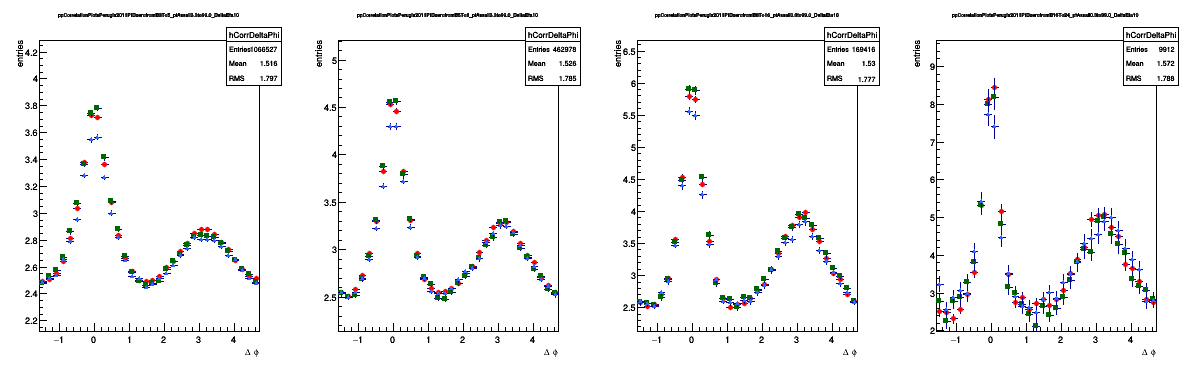
\includegraphics[width=1\linewidth]{figures/Template/1DCompare_allDpTfromB_AssoPt_0dot3to99dot0GeVc_Perugia2011.png}
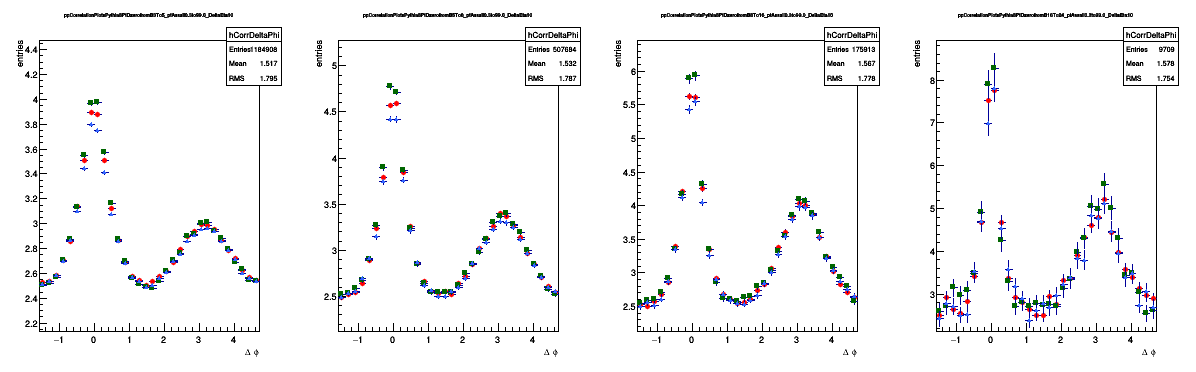
\includegraphics[width=1\linewidth]{figures/Template/1DCompare_allDpTfromB_AssoPt_0dot3to99dot0GeVc_Pythia8.png}
\caption{Azimuthal correlation distribution between D meson from b-hadron decay and charged particles obtained from Monte Carlo simulations
based on Pythia-Perugia2010 tune (row1), Pythia-Perugia2011 tune (row2), Pythia8 tune (row3) for associated track $\pt > 0.3$ GeV/c and D-meson pT ranges: 3-5, 5-8, 8-16, 16-24 GeV/c. $\Dzero$ in blue, $\Dplus$ in green, $\Dstar$ in red.}
\label{templates1}
\end{figure}

\begin{figure}
\centering
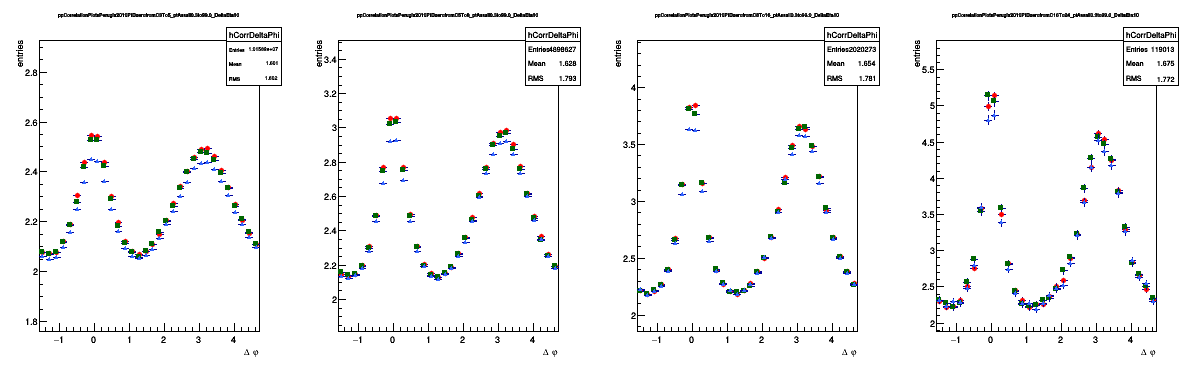
\includegraphics[width=1\linewidth]{figures/Template/1DCompare_allDpTfromC_AssoPt_0dot3to99dot0GeVc_Perugia2010.png}
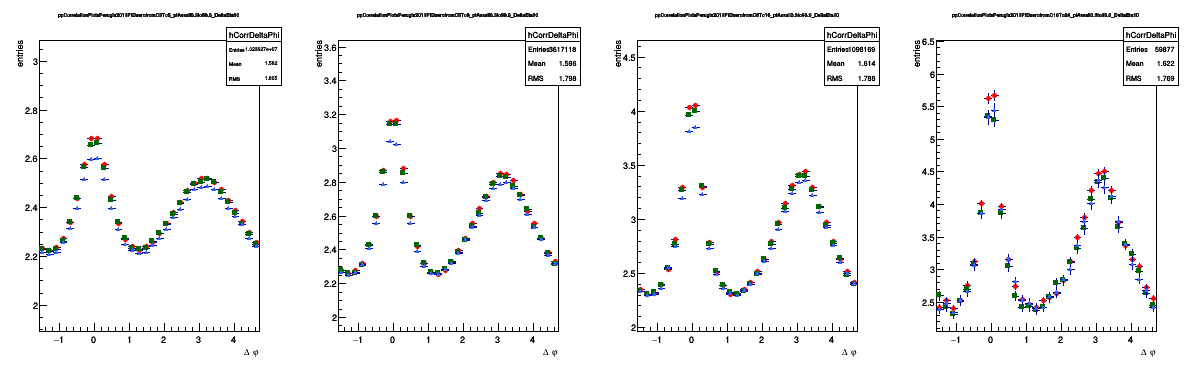
\includegraphics[width=1\linewidth]{figures/Template/1DCompare_allDpTfromC_AssoPt_0dot3to99dot0GeVc_Perugia2011.png}
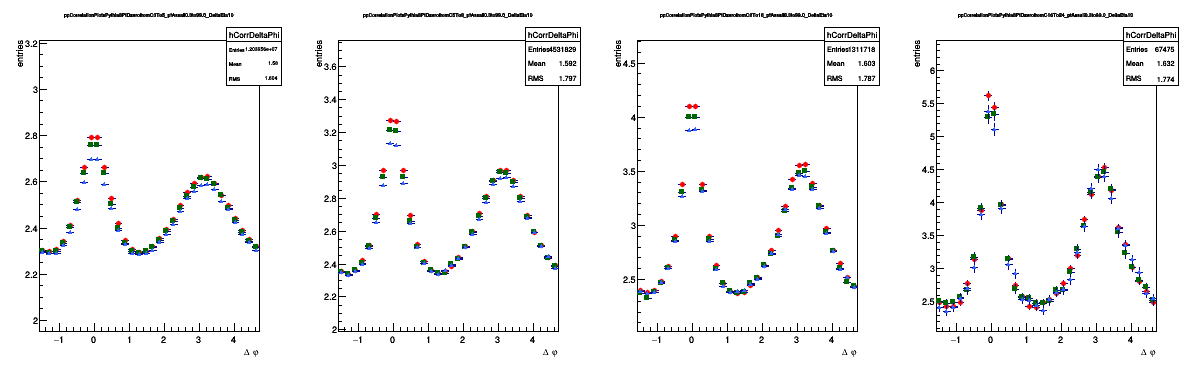
\includegraphics[width=1\linewidth]{figures/Template/1DCompare_allDpTfromC_AssoPt_0dot3to99dot0GeVc_Pythia8.png}
\caption{Azimuthal correlation distribution between prompt D meson and charged particles obtained from Monte Carlo simulations
based on Pythia-Perugia2010 tune (row1), Pythia-Perugia2011 tune (row2), Pythia8 tune (row3) for associated track $\pt > 0.3$ GeV/c and D-meson pT ranges: 3-5, 5-8, 8-16, 16-24 GeV/c. $\Dzero$ in blue, $\Dplus$ in green, $\Dstar$ in red.}
\label{templates2}
\end{figure}

The feed-down subtraction was performed after rescaling the data correlation distributions for the purity fraction, and correcting them by the near-side modulation induced by the bias on the B decay topology.

\clearpage

\newpage % always start next (sub)section with new page to avoid disarrangement.

